\documentclass[a4paper,12pt]{article}
\usepackage[margin=1.0in]{geometry}
\usepackage{setspace}
\onehalfspacing{}

\usepackage{subfiles}
\usepackage{ifthen}

% Equations
\usepackage{mathtools,amssymb,amsfonts}
\usepackage{bm, bbm}

% Images
\usepackage{graphicx}

% Table
\usepackage{booktabs}
\usepackage{multirow}
\usepackage{subcaption}
\usepackage{caption}
\usepackage{longtable}

% ekableExtra & modelsummary
\usepackage{siunitx}
\newcolumntype{d}{S[
    input-open-uncertainty=,
    input-close-uncertainty=,
    parse-numbers = false,
    table-align-text-pre=false,
    table-align-text-post=false
 ]}

% BibTeX
\usepackage[longnamesfirst]{natbib}
\usepackage{hyperref}

%% define rootfolder
\newcommand{\rootFolder}{./../..}


\begin{document}
\title{Demo}
\author{Kazuharu Yanagimoto}

\date{\today}
\maketitle

\begin{figure}
    \centering
    \caption{Number of People Hospitalized}
    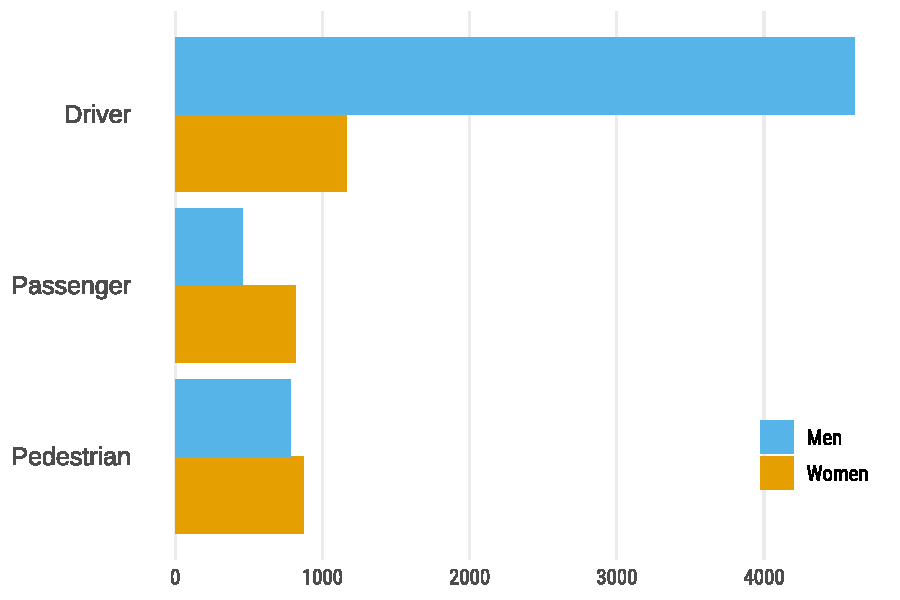
\includegraphics[width = \textwidth]{\rootFolder/output/img/num_hospitalized.pdf}
\end{figure}

\begin{figure}
    \centering
    \caption{Comparison of Themes}
    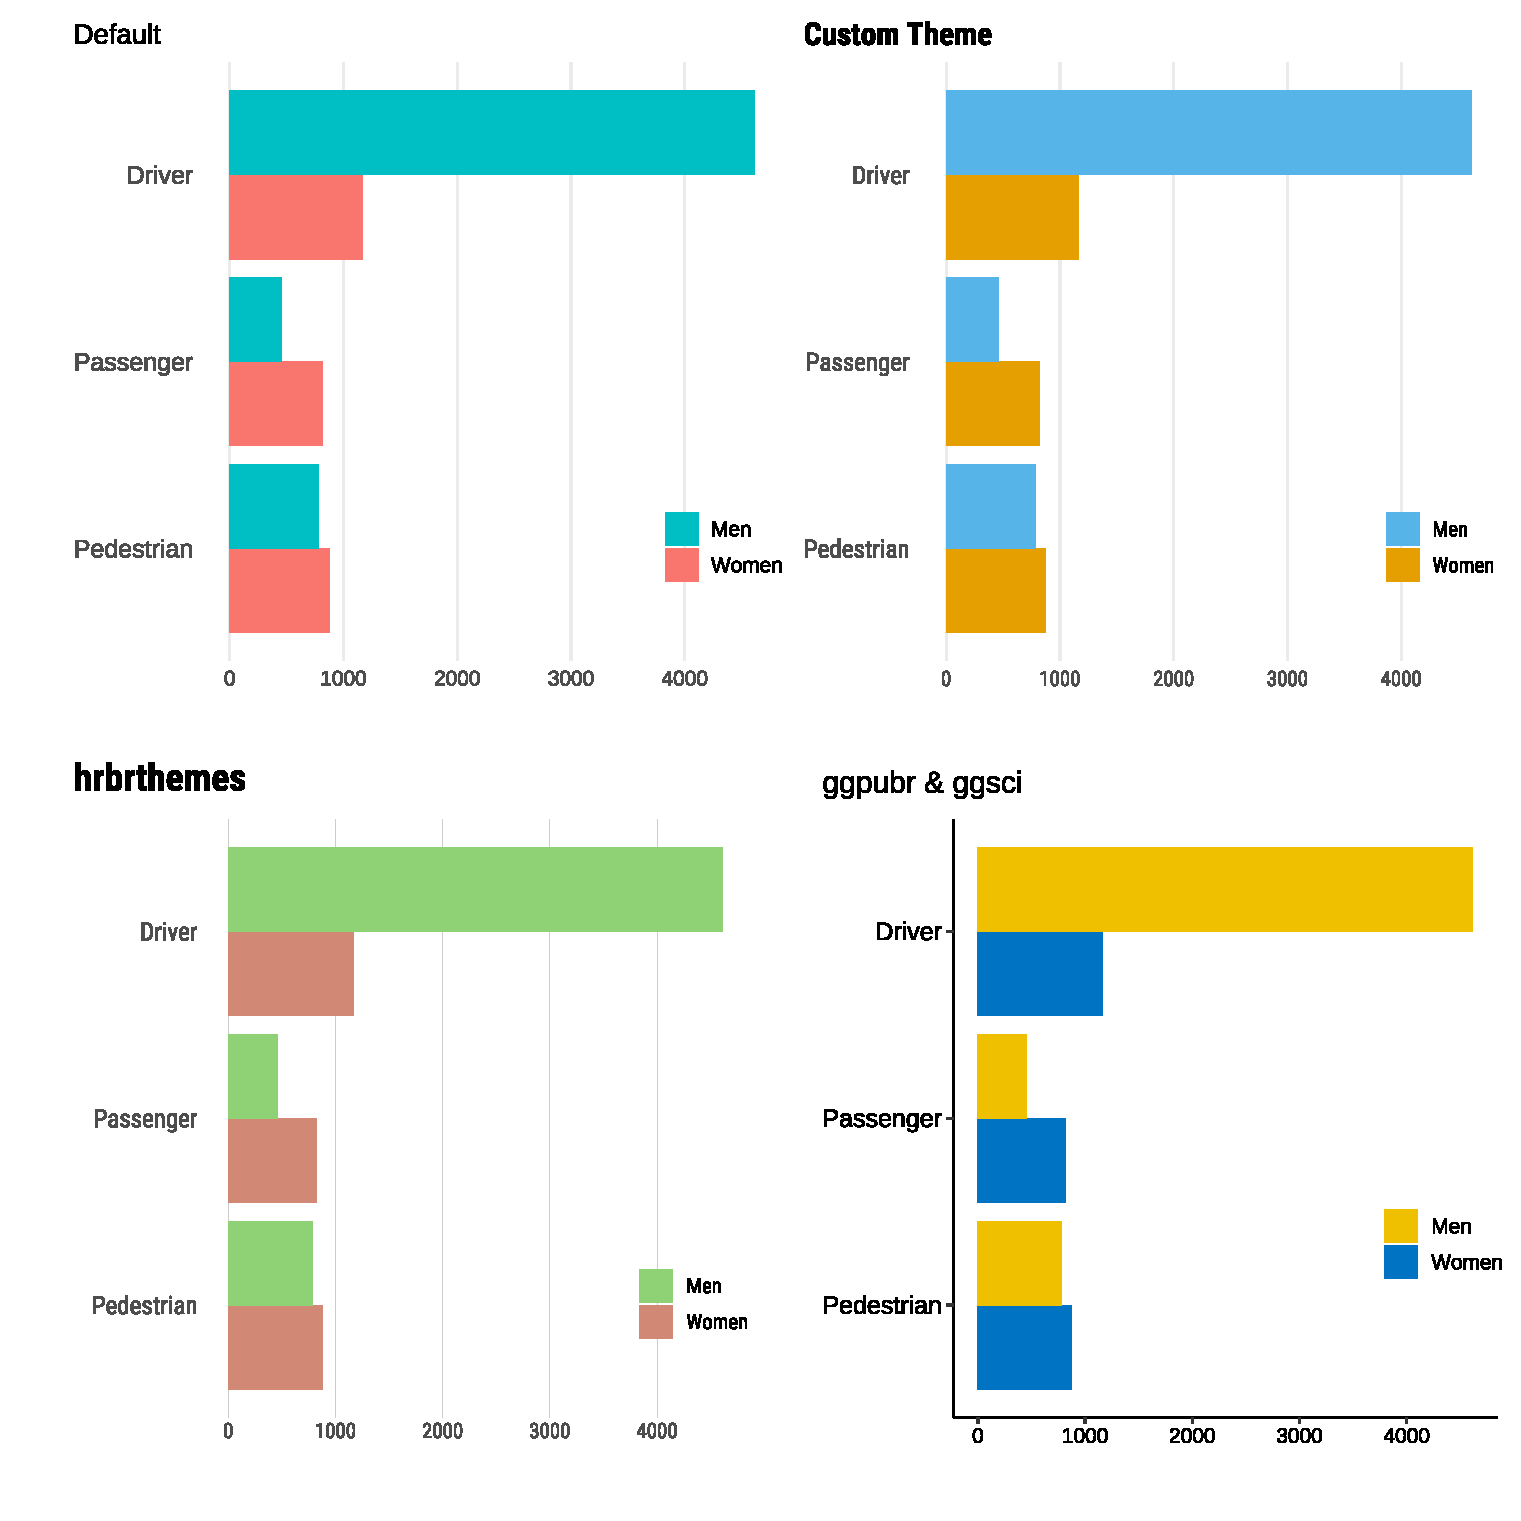
\includegraphics[width = \textwidth]{\rootFolder/output/img/comp_plots.pdf}
\end{figure}


\begin{table}
    \centering
    \caption{Number of Persons Involved in Traffic Accidents}
    
\begin{tabular}[t]{lrrrrrrrr}
\toprule
\multicolumn{1}{c}{ } & \multicolumn{4}{c}{Men} & \multicolumn{4}{c}{Women} \\
\cmidrule(l{3pt}r{3pt}){2-5} \cmidrule(l{3pt}r{3pt}){6-9}
  & 2019 & 2020 & 2021 & 2022 & 2019 & 2020 & 2021 & 2022\\
\midrule
\addlinespace[0.3em]
\multicolumn{9}{l}{\textbf{Good}}\\
\hspace{1em}sunny & 24399 & 14969 & 19208 & 19420 & 11971 & 6958 & 9417 & 9298\\
\hspace{1em}cloud & 1159 & 1190 & 1325 & 1633 & 555 & 554 & 630 & 774\\
\addlinespace[0.3em]
\multicolumn{9}{l}{\textbf{Bad}}\\
\hspace{1em}soft rain & 2126 & 1198 & 1281 & 1408 & 1068 & 542 & 605 & 716\\
\hspace{1em}hard rain & 386 & 202 & 386 & 352 & 222 & 96 & 210 & 179\\
\hspace{1em}snow & 2 & 2 & 124 & 5 &  &  & 38 & 1\\
\hspace{1em}hail & 11 & 5 & 6 & 4 & 3 & 3 & 1 & 2\\
\bottomrule
\end{tabular}

\end{table}

\begin{table}
    \centering
    \caption{Logit Regression of Hospitalization and Death within 24 Hours}
    
\begin{tabular}[t]{lcccccc}
\toprule
\multicolumn{1}{c}{ } & \multicolumn{3}{c}{Hospitalization} & \multicolumn{3}{c}{Died within 24 hours} \\
\cmidrule(l{3pt}r{3pt}){2-4} \cmidrule(l{3pt}r{3pt}){5-7}
  & (1) & (2) & (3) & (4) & (5) & (6)\\
\midrule
Positive Alcohol & \num{-0.077} & \num{0.310}** & \num{0.353}** & \num{-13.710}** & \num{-13.455}** & \num{-13.492}**\\
 & (\num{0.088}) & (\num{0.095}) & (\num{0.093}) & (\num{0.053}) & (\num{0.064}) & (\num{0.063})\\
\midrule
Observations & \num{149918} & \num{149831} & \num{134006} & \num{90852} & \num{89300} & \num{86330}\\
FE: Age Group & X & X & X & X & X & X\\
FE: Gender & X & X & X & X & X & X\\
FE: Type of Vehicle &  & X & X &  & X & X\\
FE: Weather &  &  & X &  &  & X\\
\midrule
\bottomrule
\end{tabular}

    \caption*{Notes: Passenger and pedestrian's coefficients are normalized by driver.
    **p<.01; *p<.05; +p<.1. Standard errors are clustered by age group.}
\end{table}

\end{document}
